\documentclass[10pt,a4paper]{article}
\usepackage[utf8]{inputenc}
\usepackage[english]{babel}
\usepackage[activate={true,nocompatibility},final,tracking=true,kerning=true,spacing=true]{microtype}
\usepackage{fullpage}
\usepackage{graphicx}
\usepackage{fancyhdr}
\usepackage{occi}
\setlength{\headheight}{13pt}
\pagestyle{fancy}

%  just a test
% default sans-serif
\renewcommand{\familydefault}{\sfdefault}

% no lines for headers and footers
\renewcommand{\headrulewidth}{0pt}
\renewcommand{\footrulewidth}{0pt}

% header
\fancyhf{}
\lhead{GFD-P-R.184}
\rhead{\today}

% footer
\lfoot{occi-wg@ogf.org}
\rfoot{\thepage}

% paragraphs need some space...
\setlength{\parindent}{0pt}
\setlength{\parskip}{1ex plus 0.5ex minus 0.2ex}

%\renewcommand\paragraph{%
%  \@startsection{paragraph}{4}{0mm}%
%     {-\baselineskip}%
%     {.5\baselineskip}%
%     {\normalfont\normalsize\bfseries}}

% some space between header and text...
\headsep 13pt

\setcounter{secnumdepth}{4}

\begin{document}

% header on first page is different
\thispagestyle{empty}

Draft \hfill  Thijs Metsch, Intel\\
OCCI-WG \hfill  Mohamed Mohamed, Telecom SudParis\\
\rightline {\today}

\vspace*{0.5in}

\begin{Large}
\textbf{Open Cloud Computing Interface - Platform}
\end{Large}

\vspace*{0.5in}

\underline{Status of this Document}

% This document provides information to the community regarding the
specification of the Open Cloud Computing Interface. Distribution is
unlimited.


This document is a \underline{draft} of the OCCI Platform \cite{occi:platform} specification.

\underline{Copyright Notice}

Copyright \copyright ~Open Grid Forum (2014-2015). All Rights
Reserved.

\underline{Trademarks}

OCCI is a trademark of the Open Grid Forum.

\underline{Abstract}

This document, part of a document series, produced by the OCCI working
group within the Open Grid Forum (OGF), provides a high-level
definition of a Protocol and API. The document is based upon
previously gathered requirements and focuses on the scope of important
capabilities required to support modern service offerings.


\newpage
\tableofcontents
\newpage

\section{Introduction}
The Open Cloud Computing Interface (OCCI) is a RESTful Protocol and
API for all kinds of management tasks. OCCI was originally initiated
to create a remote management API for IaaS%
\footnote{Infrastructure as a Service}
model-based services, allowing for the development of interoperable tools for
common tasks including deployment, autonomic scaling and monitoring.
%
It has since evolved into an flexible API with a strong focus on
interoperability while still offering a high degree of extensibility. The
current release of the Open Cloud Computing Interface is suitable to serve many
other models in addition to IaaS, including e.g.~PaaS and SaaS.

In order to be modular and extensible the current OCCI specification is
released as a suite of complimentary documents, which together form the complete
specification.
%
The documents are divided into three categories consisting of the OCCI Core,
the OCCI Renderings and the OCCI Extensions.
%
\begin{itemize}
\item The OCCI Core specification consists of a single document defining the
 OCCI Core Model. The OCCI Core Model can be interacted with {\em
 renderings} (including associated behaviours) and expanded through {\em extensions}.
\item The OCCI Rendering specifications consist of multiple documents each
 describing a particular rendering of the OCCI Core Model. Multiple renderings can
 interact with the same instance of the OCCI Core Model and will automatically support
 any additions to the model which follow the extension rules defined in OCCI
 Core.
\item The OCCI Extension specifications consist of multiple documents each
 describing a particular extension of the OCCI Core Model. The extension documents
 describe additions to the OCCI Core Model defined within the OCCI specification
 suite.
\end{itemize}
%
The current specification consist of three documents.
Future releases of OCCI may include additional rendering and extension
specifications. The documents of the current OCCI specification suite are:

\begin{description}
\item[OCCI Core] describes the formal definition of the the OCCI Core Model
\cite{occi:core}.
\item[OCCI HTTP Rendering] defines how to interact with the OCCI Core Model using the
RESTful OCCI API \cite{occi:http_rendering}. The document defines how the OCCI Core Model can
be communicated and thus serialised using the HTTP protocol.
\item[OCCI Infrastructure] contains the definition of the OCCI Infrastructure
extension for the IaaS domain \cite{occi:infrastructure}. The document defines
additional resource types, their attributes and the actions that can be taken
on each resource type.
\end{description}


OCCI makes an ideal interoperable boundary interface between the web
and the internal resource management system of platform providers.

\section{Notational Conventions}
All these parts and the information within are mandatory for
implementors (unless otherwise specified). The key words "MUST", "MUST
NOT", "REQUIRED", "SHALL", "SHALL NOT", "SHOULD", "SHOULD NOT",
"RECOMMENDED", "MAY", and "OPTIONAL" in this document are to be
interpreted as described in RFC 2119 \cite{rfc2119}.

\textbf{Andy: we need to state that this document as part of the current document set,
supersedes all previous documents.}


% begin platform content

\section{Platform}

The OCCI Platform document details how an OCCI implementation can model and implement a Platform as a Service API offering by extending the OCCI Core Model. This API enables the provisioning and management of PaaS resources. For example, it allows to deploy an application on one or more PaaS components. The application itself could be composed of different Components. The main platform types defined within OCCI Platform are:

\begin{description}
  \item[Application] Which defines the user-defined part of the overall service.
  \item[Component] A configured instance of a piece of code providing business functions that are part of the execution of the application or responsible of hosting the application.
  \item[ComponentLink] Connects an Application instance to a hosting Component or connects two components.
\end{description}

\begin{figure}[!h]
	{\centering \resizebox*{0.7\columnwidth}{!}{\rotatebox{0}
	{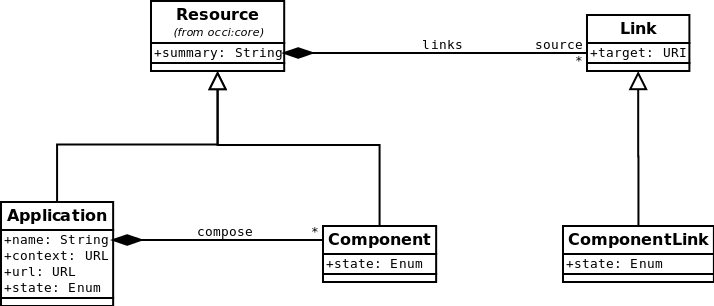
\includegraphics[scale=0.4]{figs/platform_overview.png}}} \par}
	\caption{Overview Diagram of OCCI Platform Types.}
	\label{fig:platform_uml}
\end{figure}

These platform types inherit the OCCI Core Model Resource base type and all their attributes. One can use the HTTP Protocol and suitable rendering to discover and consume these resources. Independently of the implementation, the defined resources could be discoverable during runtime through OCCI compliant interfaces.

As REQUIRED by the OCCI Core Model specification, every type instantiated that is a  sub-type of \hl{Resource} or \hl{Link} MUST be assigned a Kind that identifies the instantiated type. Each such Kind instance MUST be related to the Resource or Link base type's Kind. That assigned Kind instance MUST always remain immutable to any client.

\subsection{Application Kind Definition}
The following kind MUST be present and represents the kind definition of an application resource. 

\hl{Application} inherits the \hl{Resource} base type defined in OCCI Core Model \cite{occi:core}. \hl{Application} is assigned the \hl{Kind} instance \textit{http://schemas.ogf.org/occi/platform\#application}. A \hl{Application} instance MUST use and expose this \hl{Kind}.

\mytablefloat{
	\label{tbl:app}\hl{Attribute}s defined for the \hl{Application} type.
}
{
	\begin{tabular}{lp{2.5cm}p{1cm}lp{5cm}}
	\toprule
	Attribute&Type&Multi\-plicity&Mutability&Description\\
	\colrule
	occi.app.name & String & 1 & Mutable & Name of the application.\\
	occi.app.context & URL & 1 & Immutable & URL for contextualizing the app.\\
	occi.app.url & URL & 1 & Immutable & DNS entry.\\
	occi.app.state & Enum \{active, inactive, error\} & 1 & Immutable & State of the application.\\
	occi.app.state.message & String & 0..1 & Immutable & Human-readable explanation of the current instance state.
	\botrule
	\end{tabular}
}

Table~\ref{tbl:app} describes the Attributes defined by \hl{Application} instance. These attributes MAY or MUST be exposed by an instance of the \hl{Application} type depending on the ``Multiplicity'' column in the aforementioned table.

The \hl{Action}s are defined by the \hl{Kind} instance \textit{http://schemas.ogf.org/occi/platform\#application}. Every \hl{Action} instance in the table uses the\textit{http://schemas.ogf.org/occi/platform/action\#} categorisation scheme. ``Action Term'' below refers to \hl{Action}.{\tt term}

\mytablefloat{
	\label{tbl:app_actions}
	\hl{Action}s applicable to instances of the \hl{Application} type.
}
{
	\begin{tabular}{lll}
	\toprule
	Action Term & Target state & Attributes \\
	\colrule
	start & active & -- \\
	stop & inactive & -- \\
	\botrule
	\end{tabular}
}

The state model for the \hl{Application} instance is defined in \ref{fig:app_state}:

\begin{figure}[!h]
	{\centering \resizebox*{0.5\columnwidth}{!}{\rotatebox{0}
	{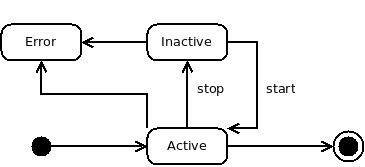
\includegraphics[scale=0.2]{figs/platform_component_state.png}}} \par}
	\caption{State model of a \hl{Application} instance.}
	\label{fig:app_state}
\end{figure}

\subsection{Component Kind Definition}
The following kind MUST be present and represents the kind definition of an component resource. 

\hl{Component} inherits the \hl{Resource} base type defined in OCCI Core Model \cite{occi:core}. \hl{Application} is assigned the \hl{Kind} instance \textit{http://schemas.ogf.org/occi/platform\#component}. A \hl{Component} instance MUST use and expose this \hl{Kind}.

\mytablefloat{
	\label{tbl:component}\hl{Attribute}s defined for the \hl{Component} type.
}
{
	\begin{tabular}{lp{2.5cm}p{1cm}lp{5cm}}
	\toprule
	Attribute&Type&Multi\-plicity&Mutability&Description\\
	\colrule
	occi.component.state & Enum \{active, inactive, error\} & 1 & Immutable & State of the component.\\
	occi.component.state.message & String & 0..1 & Immutable & Human-readable explanation of the current instance state.
	\botrule
	\end{tabular}
}

Table~\ref{tbl:component} describes the Attributes defined by \hl{Component} instance. These attributes MAY or MUST be exposed by an instance of the \hl{Component} type depending on the ``Multiplicity'' column in the aforementioned table.

The \hl{Action}s are defined by the \hl{Kind} instance \textit{http://schemas.ogf.org/occi/platform\#Component}. Every \hl{Action} instance in the table uses the\textit{http://schemas.ogf.org/occi/platform/action\#} categorisation scheme. ``Action Term'' below refers to \hl{Action}.{\tt term}

\mytablefloat{
	\label{tbl:component_actions}
	\hl{Action}s applicable to instances of the \hl{Application} type.
}
{
	\begin{tabular}{lll}
	\toprule
	Action Term & Target state & Attributes \\
	\colrule
	start & active & -- \\
	stop & inactive & -- \\
	\botrule
	\end{tabular}
}

The state model for the \hl{Component} instance is defined in \ref{fig:component_state}:

\begin{figure}[!h]
	{\centering \resizebox*{0.5\columnwidth}{!}{\rotatebox{0}
	{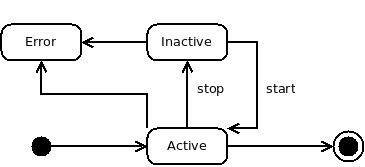
\includegraphics[scale=0.2]{figs/platform_component_state.png}}} \par}
	\caption{State model of a \hl{Component} instance.}
	\label{fig:component_state}
\end{figure}

\subsection{Linking to Components}

The composition of a service is realized through the linkage of \hl{Application} and \hl{Component} instances with each other. 

\hl{ComponentLink} inherits the \hl{Link} base type defined in OCCI Core Model \cite{occi:core}. \hl{ComponentLink} is assigned the \hl{Kind} instance \textit{http://schemas.ogf.org/occi/platform\#componentLink}. The \hl{Kind} instance assigned to the \hl{ComponentLink} type MUST be related to the \textit{http://schemas.ogf.org/occi/core\#link} \hl{Kind} by setting the \textit{parent} attribute.

The componentLink kind can be further enhanced by the use of  provider specific Mixins. This can be used to expose details such as databased access URIs for an application linked up with a database component.

\subsection{Platform Templates}
Platform Templates allow for clients of an OCCI implementation to quickly and conveniently apply predefined configurations to OCCI Platform defined types. They are implemented using Mixin instances. There are two supported platform templates types in OCCI Platform.

\subsubsection{Application Template}
Application templates allow clients to define which underlying framework the application should use (e.g. Programming language). 

The Application Template is defined by a Mixin. A provider specific defined Application Template Mixin MUST relate to the OCCI Application Template Mixin in order to give absolute type information. The OCCI Application Template is defined by the \textit{http://schemas.ogf.org/occi/platform\#app\_tpl} Mixin and MUST be supported SHOULD Application Templates be offered.

Provider specific Application Templates are constructed using a “term” and “scheme” combination. Where the “term” is a provider specific description of the framework (e.g. python, ruby, …). Where an implementation requires additional information to be hold in the Templates Mixin, it MAY do so by using Category’s inherited Attributes.

\subsubsection{Resource Template}
The Resource Template Mixin builds upon the concept of Application Templates. A Resource Template is a provider defined Mixin instance that refers to a preset Resource configuration.

This can be used to define the resource instance attributes of the application and component. The provider specific resource Templates are defined by using a "term" and "scheme" combination. Those provider specific Resource Template Mixin must relate to the OCCI Resource Template defined by \textit{http://schemas.ogf.org/occi/platform\#res\_tpl}. Where an implementation requires additional information to be hold in the Templates Mixin, it MAY do so by using Category’s inherited Attributes.

An example of these templates is shown in the following UML diagram in Figure \ref{fig:templates}.

\begin{figure}[!h]
	{\centering \resizebox*{0.7\columnwidth}{!}{\rotatebox{0}
	{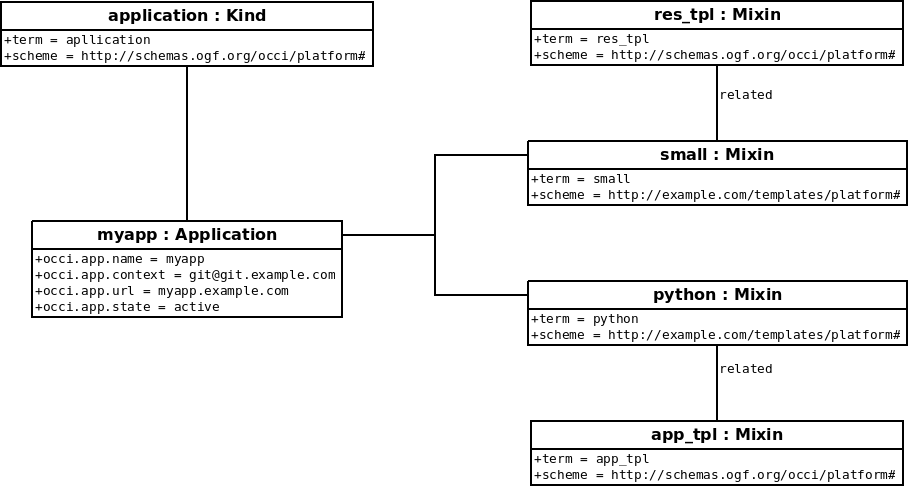
\includegraphics[scale=0.5]{figs/platform_templates.png}}} \par}
	\caption{Application and Resource Templates.}
	\label{fig:templates}
\end{figure}

\section{Specific Component Instance Mixins}
The following sections describe \hl{Mixin}s instances which SHOULD be implemented by Providers for some basic component type.

\subsection{Database Mixin}

\hl{Database} inherits the \hl{Mixin} base type defined in OCCI Core Model \cite{occi:core}. \hl{Database} is assigned the \hl{Mixin} instance \textit{http://schemas.ogf.org/occi/platform\#database}. The \hl{Database} instance applies to the \hl{Component} instance defined above.

\mytablefloat{
	\label{tbl:database}\hl{Attribute}s defined for the \hl{Database} type.
}
{
	\begin{tabular}{lp{2.5cm}p{1cm}lp{5cm}}
	\toprule
	Attribute&Type&Multi\-plicity&Mutability&Description\\
	\colrule
	occi.database.version & String & 1 & Immutable & Version of the database.\\
	\botrule
	\end{tabular}
}

Table~\ref{tbl:database} describes the Attributes defined by \hl{Database} instance. 

\subsubsection{Database Link}
In case that a \hl{Application} instance links to a \hl{Component} instance which has the \hl{Database} \hl{Mixin} instance applied the following \hl{Mixin} SHOULD be applied to the \hl{ComponentLink}.

\hl{DatabaseLink} inherits the \hl{Mixin} base type defined in OCCI Core Model \cite{occi:core}. \hl{DatabaseLink} is assigned the \hl{Mixin} instance \textit{http://schemas.ogf.org/occi/platform\#databaseLink}. The \hl{DatabaseLink} instance applies to the \hl{ComponentLink} instance defined above.

\mytablefloat{
	\label{tbl:database_link}\hl{Attribute}s defined for the \hl{Database} type.
}
{
	\begin{tabular}{lp{2.5cm}p{1cm}lp{5cm}}
	\toprule
	Attribute&Type&Multi\-plicity&Mutability&Description\\
	\colrule
	occi.database.uri & URI & 1 & Immutable & Connection URI for the database instance.\\
	occi.database.username & URI & 0\ldots1 & Immutable & Username.\\
	occi.database.token & URI & 0\ldots1 & Immutable & Token.\\
	\botrule
	\end{tabular}
}

Table~\ref{tbl:database_link} describes the Attributes defined by \hl{DatabaseLink} instance. 

% end platform content

\section{Security Considerations}
The OCCI Platform specification is an extension to the OCCI Core
and Model specification \cite{occi:core}; thus the same security
considerations as for the OCCI Core and Model specification apply
here.

\section{Glossary}
\label{sec:glossary}
\begin{tabular}{l|p{12cm}}
Term & Description \\
\hline
\hl{Action} & An OCCI base type. Represent an invocable operation on a \hl{Entity} sub-type instance or collection thereof. \\

\hl{Category} & A type in the OCCI model. The parent type of \hl{Kind}. \\

\hl{Client} & An OCCI client.\\

\hl{Collection} & A set of \hl{Entity} sub-type instances all associated to a particular \hl{Kind} or \hl{Mixin} instance. \\

\hl{Entity} & An OCCI base type. The parent type of \hl{Resource} and \hl{Link}. \\

\hl{Kind} & A type in the OCCI model. A core component of the OCCI classification system. \\

\hl{Link} & An OCCI base type. A \hl{Link} instance associate one \hl{Resource} instance with another. \\

mixin & An instance of the \hl{Mixin} type associated with a {\bf resource
 instance}. The ``mixin'' concept as used by OCCI {\em only} applies to
 instances, never to \hl{Entity} types. \\

\hl{Mixin} & A type in the OCCI model. A core component of the OCCI classification system. \\

\hl{OCCI} & Open Cloud Computing Interface \\

OCCI base type & One of \hl{Entity}, \hl{Resource}, \hl{Link} or \hl{Action}. \\

OGF & Open Grid Forum \\

\hl{Resource} & An OCCI base type. The parent type for all domain-specific resource types. \\

resource instance & An instance of a sub-type of \hl{Entity}. The OCCI
 model defines two sub-types of \hl{Entity}, the \hl{Resource} type and the
 \hl{Link} type. However, the term {\em resource instance} is defined to
 include any instance of a {\em sub-type} of \hl{Resource} or \hl{Link} as
 well. \\

Tag & A \hl{Mixin} instance with no attributes or actions defined. \\

Template & A \hl{Mixin} instance which if associated at resource instantiation
time pre-populate certain attributes. \\

type & One of the types defined by the OCCI model.  The OCCI model types are
 \hl{Category}, \hl{Kind}, \hl{Mixin}, \hl{Action}, \hl{Entity}, \hl{Resource}
 and \hl{Link}. \\

URI & Uniform Resource Identifier \\
URL & Uniform Resource Locator \\
URN & Uniform Resource Name \\
\end{tabular}


\section{Contributors}
We would like to thank the following people who contributed to this
document:

\begin{tabular}{l|p{2in}|p{2in}}
Name & Affiliation & Contact \\
\hline
Andy Edmonds & ICCLab, ZHAW & edmo at zhaw.ch \\
Peter Troeger & TU Chemnitz & peter@troeger.eu \\
Thijs Metsch & Intel & thijs.metsch@intel.com\\
Sami Yangui & & \\
Mohamed Mohamed & Telecom SudParis & \\
\end{tabular}

Next to these individual contributions we value the contributions from
the OCCI working group.

\section{Intellectual Property Statement}
The OGF takes no position regarding the validity or scope of any
intellectual property or other rights that might be claimed to pertain
to the implementation or use of the technology described in this
document or the extent to which any license under such rights might or
might not be available; neither does it represent that it has made any
effort to identify any such rights. Copies of claims of rights made
available for publication and any assurances of licenses to be made
available, or the result of an attempt made to obtain a general
license or permission for the use of such proprietary rights by
implementers or users of this specification can be obtained from the
OGF Secretariat.

The OGF invites any interested party to bring to its attention any
copyrights, patents or patent applications, or other proprietary
rights which may cover technology that may be required to practice
this recommendation. Please address the information to the OGF
Executive Director.


\section{Disclaimer}
This document and the information contained herein is provided on an
``As Is'' basis and the OGF disclaims all warranties, express or
implied, including but not limited to any warranty that the use of the
information herein will not infringe any rights or any implied
warranties of merchantability or fitness for a particular purpose.


\section{Full Copyright Notice}
Copyright \copyright ~Open Grid Forum (2009-2014). All Rights Reserved.

This document and translations of it may be copied and furnished to
others, and derivative works that comment on or otherwise explain it
or assist in its implementation may be prepared, copied, published and
distributed, in whole or in part, without restriction of any kind,
provided that the above copyright notice and this paragraph are
included on all such copies and derivative works. However, this
document itself may not be modified in any way, such as by removing
the copyright notice or references to the OGF or other organizations,
except as needed for the purpose of developing Grid Recommendations in
which case the procedures for copyrights defined in the OGF Document
process must be followed, or as required to translate it into
languages other than English.

The limited permissions granted above are perpetual and will not be
revoked by the OGF or its successors or assignees.


\bibliographystyle{IEEEtran}
\bibliography{references}

\end{document}
